\documentclass[11pt]{article}

    \usepackage[breakable]{tcolorbox}
    \usepackage{parskip} % Stop auto-indenting (to mimic markdown behaviour)
    
    \usepackage{iftex}
    \ifPDFTeX
    	\usepackage[T1]{fontenc}
    	\usepackage{mathpazo}
    \else
    	\usepackage{fontspec}
    \fi

    % Basic figure setup, for now with no caption control since it's done
    % automatically by Pandoc (which extracts ![](path) syntax from Markdown).
    \usepackage{graphicx}
    % Maintain compatibility with old templates. Remove in nbconvert 6.0
    \let\Oldincludegraphics\includegraphics
    % Ensure that by default, figures have no caption (until we provide a
    % proper Figure object with a Caption API and a way to capture that
    % in the conversion process - todo).
    \usepackage{caption}
    \DeclareCaptionFormat{nocaption}{}
    \captionsetup{format=nocaption,aboveskip=0pt,belowskip=0pt}

    \usepackage{float}
    \floatplacement{figure}{H} % forces figures to be placed at the correct location
    \usepackage{xcolor} % Allow colors to be defined
    \usepackage{enumerate} % Needed for markdown enumerations to work
    \usepackage{geometry} % Used to adjust the document margins
    \usepackage{amsmath} % Equations
    \usepackage{amssymb} % Equations
    \usepackage{textcomp} % defines textquotesingle
    % Hack from http://tex.stackexchange.com/a/47451/13684:
    \AtBeginDocument{%
        \def\PYZsq{\textquotesingle}% Upright quotes in Pygmentized code
    }
    \usepackage{upquote} % Upright quotes for verbatim code
    \usepackage{eurosym} % defines \euro
    \usepackage[mathletters]{ucs} % Extended unicode (utf-8) support
    \usepackage{fancyvrb} % verbatim replacement that allows latex
    \usepackage{grffile} % extends the file name processing of package graphics 
                         % to support a larger range
    \makeatletter % fix for old versions of grffile with XeLaTeX
    \@ifpackagelater{grffile}{2019/11/01}
    {
      % Do nothing on new versions
    }
    {
      \def\Gread@@xetex#1{%
        \IfFileExists{"\Gin@base".bb}%
        {\Gread@eps{\Gin@base.bb}}%
        {\Gread@@xetex@aux#1}%
      }
    }
    \makeatother
    \usepackage[Export]{adjustbox} % Used to constrain images to a maximum size
    \adjustboxset{max size={0.9\linewidth}{0.9\paperheight}}

    % The hyperref package gives us a pdf with properly built
    % internal navigation ('pdf bookmarks' for the table of contents,
    % internal cross-reference links, web links for URLs, etc.)
    \usepackage{hyperref}
    % The default LaTeX title has an obnoxious amount of whitespace. By default,
    % titling removes some of it. It also provides customization options.
    \usepackage{titling}
    \usepackage{longtable} % longtable support required by pandoc >1.10
    \usepackage{booktabs}  % table support for pandoc > 1.12.2
    \usepackage[inline]{enumitem} % IRkernel/repr support (it uses the enumerate* environment)
    \usepackage[normalem]{ulem} % ulem is needed to support strikethroughs (\sout)
                                % normalem makes italics be italics, not underlines
    \usepackage{mathrsfs}
    

    
    % Colors for the hyperref package
    \definecolor{urlcolor}{rgb}{0,.145,.698}
    \definecolor{linkcolor}{rgb}{.71,0.21,0.01}
    \definecolor{citecolor}{rgb}{.12,.54,.11}

    % ANSI colors
    \definecolor{ansi-black}{HTML}{3E424D}
    \definecolor{ansi-black-intense}{HTML}{282C36}
    \definecolor{ansi-red}{HTML}{E75C58}
    \definecolor{ansi-red-intense}{HTML}{B22B31}
    \definecolor{ansi-green}{HTML}{00A250}
    \definecolor{ansi-green-intense}{HTML}{007427}
    \definecolor{ansi-yellow}{HTML}{DDB62B}
    \definecolor{ansi-yellow-intense}{HTML}{B27D12}
    \definecolor{ansi-blue}{HTML}{208FFB}
    \definecolor{ansi-blue-intense}{HTML}{0065CA}
    \definecolor{ansi-magenta}{HTML}{D160C4}
    \definecolor{ansi-magenta-intense}{HTML}{A03196}
    \definecolor{ansi-cyan}{HTML}{60C6C8}
    \definecolor{ansi-cyan-intense}{HTML}{258F8F}
    \definecolor{ansi-white}{HTML}{C5C1B4}
    \definecolor{ansi-white-intense}{HTML}{A1A6B2}
    \definecolor{ansi-default-inverse-fg}{HTML}{FFFFFF}
    \definecolor{ansi-default-inverse-bg}{HTML}{000000}

    % common color for the border for error outputs.
    \definecolor{outerrorbackground}{HTML}{FFDFDF}

    % commands and environments needed by pandoc snippets
    % extracted from the output of `pandoc -s`
    \providecommand{\tightlist}{%
      \setlength{\itemsep}{0pt}\setlength{\parskip}{0pt}}
    \DefineVerbatimEnvironment{Highlighting}{Verbatim}{commandchars=\\\{\}}
    % Add ',fontsize=\small' for more characters per line
    \newenvironment{Shaded}{}{}
    \newcommand{\KeywordTok}[1]{\textcolor[rgb]{0.00,0.44,0.13}{\textbf{{#1}}}}
    \newcommand{\DataTypeTok}[1]{\textcolor[rgb]{0.56,0.13,0.00}{{#1}}}
    \newcommand{\DecValTok}[1]{\textcolor[rgb]{0.25,0.63,0.44}{{#1}}}
    \newcommand{\BaseNTok}[1]{\textcolor[rgb]{0.25,0.63,0.44}{{#1}}}
    \newcommand{\FloatTok}[1]{\textcolor[rgb]{0.25,0.63,0.44}{{#1}}}
    \newcommand{\CharTok}[1]{\textcolor[rgb]{0.25,0.44,0.63}{{#1}}}
    \newcommand{\StringTok}[1]{\textcolor[rgb]{0.25,0.44,0.63}{{#1}}}
    \newcommand{\CommentTok}[1]{\textcolor[rgb]{0.38,0.63,0.69}{\textit{{#1}}}}
    \newcommand{\OtherTok}[1]{\textcolor[rgb]{0.00,0.44,0.13}{{#1}}}
    \newcommand{\AlertTok}[1]{\textcolor[rgb]{1.00,0.00,0.00}{\textbf{{#1}}}}
    \newcommand{\FunctionTok}[1]{\textcolor[rgb]{0.02,0.16,0.49}{{#1}}}
    \newcommand{\RegionMarkerTok}[1]{{#1}}
    \newcommand{\ErrorTok}[1]{\textcolor[rgb]{1.00,0.00,0.00}{\textbf{{#1}}}}
    \newcommand{\NormalTok}[1]{{#1}}
    
    % Additional commands for more recent versions of Pandoc
    \newcommand{\ConstantTok}[1]{\textcolor[rgb]{0.53,0.00,0.00}{{#1}}}
    \newcommand{\SpecialCharTok}[1]{\textcolor[rgb]{0.25,0.44,0.63}{{#1}}}
    \newcommand{\VerbatimStringTok}[1]{\textcolor[rgb]{0.25,0.44,0.63}{{#1}}}
    \newcommand{\SpecialStringTok}[1]{\textcolor[rgb]{0.73,0.40,0.53}{{#1}}}
    \newcommand{\ImportTok}[1]{{#1}}
    \newcommand{\DocumentationTok}[1]{\textcolor[rgb]{0.73,0.13,0.13}{\textit{{#1}}}}
    \newcommand{\AnnotationTok}[1]{\textcolor[rgb]{0.38,0.63,0.69}{\textbf{\textit{{#1}}}}}
    \newcommand{\CommentVarTok}[1]{\textcolor[rgb]{0.38,0.63,0.69}{\textbf{\textit{{#1}}}}}
    \newcommand{\VariableTok}[1]{\textcolor[rgb]{0.10,0.09,0.49}{{#1}}}
    \newcommand{\ControlFlowTok}[1]{\textcolor[rgb]{0.00,0.44,0.13}{\textbf{{#1}}}}
    \newcommand{\OperatorTok}[1]{\textcolor[rgb]{0.40,0.40,0.40}{{#1}}}
    \newcommand{\BuiltInTok}[1]{{#1}}
    \newcommand{\ExtensionTok}[1]{{#1}}
    \newcommand{\PreprocessorTok}[1]{\textcolor[rgb]{0.74,0.48,0.00}{{#1}}}
    \newcommand{\AttributeTok}[1]{\textcolor[rgb]{0.49,0.56,0.16}{{#1}}}
    \newcommand{\InformationTok}[1]{\textcolor[rgb]{0.38,0.63,0.69}{\textbf{\textit{{#1}}}}}
    \newcommand{\WarningTok}[1]{\textcolor[rgb]{0.38,0.63,0.69}{\textbf{\textit{{#1}}}}}
    
    
    % Define a nice break command that doesn't care if a line doesn't already
    % exist.
    \def\br{\hspace*{\fill} \\* }
    % Math Jax compatibility definitions
    \def\gt{>}
    \def\lt{<}
    \let\Oldtex\TeX
    \let\Oldlatex\LaTeX
    \renewcommand{\TeX}{\textrm{\Oldtex}}
    \renewcommand{\LaTeX}{\textrm{\Oldlatex}}
    % Document parameters
    % Document title
    \title{3.2 Velocity-based motion model}
    
    
    
    
    
% Pygments definitions
\makeatletter
\def\PY@reset{\let\PY@it=\relax \let\PY@bf=\relax%
    \let\PY@ul=\relax \let\PY@tc=\relax%
    \let\PY@bc=\relax \let\PY@ff=\relax}
\def\PY@tok#1{\csname PY@tok@#1\endcsname}
\def\PY@toks#1+{\ifx\relax#1\empty\else%
    \PY@tok{#1}\expandafter\PY@toks\fi}
\def\PY@do#1{\PY@bc{\PY@tc{\PY@ul{%
    \PY@it{\PY@bf{\PY@ff{#1}}}}}}}
\def\PY#1#2{\PY@reset\PY@toks#1+\relax+\PY@do{#2}}

\expandafter\def\csname PY@tok@w\endcsname{\def\PY@tc##1{\textcolor[rgb]{0.73,0.73,0.73}{##1}}}
\expandafter\def\csname PY@tok@c\endcsname{\let\PY@it=\textit\def\PY@tc##1{\textcolor[rgb]{0.25,0.50,0.50}{##1}}}
\expandafter\def\csname PY@tok@cp\endcsname{\def\PY@tc##1{\textcolor[rgb]{0.74,0.48,0.00}{##1}}}
\expandafter\def\csname PY@tok@k\endcsname{\let\PY@bf=\textbf\def\PY@tc##1{\textcolor[rgb]{0.00,0.50,0.00}{##1}}}
\expandafter\def\csname PY@tok@kp\endcsname{\def\PY@tc##1{\textcolor[rgb]{0.00,0.50,0.00}{##1}}}
\expandafter\def\csname PY@tok@kt\endcsname{\def\PY@tc##1{\textcolor[rgb]{0.69,0.00,0.25}{##1}}}
\expandafter\def\csname PY@tok@o\endcsname{\def\PY@tc##1{\textcolor[rgb]{0.40,0.40,0.40}{##1}}}
\expandafter\def\csname PY@tok@ow\endcsname{\let\PY@bf=\textbf\def\PY@tc##1{\textcolor[rgb]{0.67,0.13,1.00}{##1}}}
\expandafter\def\csname PY@tok@nb\endcsname{\def\PY@tc##1{\textcolor[rgb]{0.00,0.50,0.00}{##1}}}
\expandafter\def\csname PY@tok@nf\endcsname{\def\PY@tc##1{\textcolor[rgb]{0.00,0.00,1.00}{##1}}}
\expandafter\def\csname PY@tok@nc\endcsname{\let\PY@bf=\textbf\def\PY@tc##1{\textcolor[rgb]{0.00,0.00,1.00}{##1}}}
\expandafter\def\csname PY@tok@nn\endcsname{\let\PY@bf=\textbf\def\PY@tc##1{\textcolor[rgb]{0.00,0.00,1.00}{##1}}}
\expandafter\def\csname PY@tok@ne\endcsname{\let\PY@bf=\textbf\def\PY@tc##1{\textcolor[rgb]{0.82,0.25,0.23}{##1}}}
\expandafter\def\csname PY@tok@nv\endcsname{\def\PY@tc##1{\textcolor[rgb]{0.10,0.09,0.49}{##1}}}
\expandafter\def\csname PY@tok@no\endcsname{\def\PY@tc##1{\textcolor[rgb]{0.53,0.00,0.00}{##1}}}
\expandafter\def\csname PY@tok@nl\endcsname{\def\PY@tc##1{\textcolor[rgb]{0.63,0.63,0.00}{##1}}}
\expandafter\def\csname PY@tok@ni\endcsname{\let\PY@bf=\textbf\def\PY@tc##1{\textcolor[rgb]{0.60,0.60,0.60}{##1}}}
\expandafter\def\csname PY@tok@na\endcsname{\def\PY@tc##1{\textcolor[rgb]{0.49,0.56,0.16}{##1}}}
\expandafter\def\csname PY@tok@nt\endcsname{\let\PY@bf=\textbf\def\PY@tc##1{\textcolor[rgb]{0.00,0.50,0.00}{##1}}}
\expandafter\def\csname PY@tok@nd\endcsname{\def\PY@tc##1{\textcolor[rgb]{0.67,0.13,1.00}{##1}}}
\expandafter\def\csname PY@tok@s\endcsname{\def\PY@tc##1{\textcolor[rgb]{0.73,0.13,0.13}{##1}}}
\expandafter\def\csname PY@tok@sd\endcsname{\let\PY@it=\textit\def\PY@tc##1{\textcolor[rgb]{0.73,0.13,0.13}{##1}}}
\expandafter\def\csname PY@tok@si\endcsname{\let\PY@bf=\textbf\def\PY@tc##1{\textcolor[rgb]{0.73,0.40,0.53}{##1}}}
\expandafter\def\csname PY@tok@se\endcsname{\let\PY@bf=\textbf\def\PY@tc##1{\textcolor[rgb]{0.73,0.40,0.13}{##1}}}
\expandafter\def\csname PY@tok@sr\endcsname{\def\PY@tc##1{\textcolor[rgb]{0.73,0.40,0.53}{##1}}}
\expandafter\def\csname PY@tok@ss\endcsname{\def\PY@tc##1{\textcolor[rgb]{0.10,0.09,0.49}{##1}}}
\expandafter\def\csname PY@tok@sx\endcsname{\def\PY@tc##1{\textcolor[rgb]{0.00,0.50,0.00}{##1}}}
\expandafter\def\csname PY@tok@m\endcsname{\def\PY@tc##1{\textcolor[rgb]{0.40,0.40,0.40}{##1}}}
\expandafter\def\csname PY@tok@gh\endcsname{\let\PY@bf=\textbf\def\PY@tc##1{\textcolor[rgb]{0.00,0.00,0.50}{##1}}}
\expandafter\def\csname PY@tok@gu\endcsname{\let\PY@bf=\textbf\def\PY@tc##1{\textcolor[rgb]{0.50,0.00,0.50}{##1}}}
\expandafter\def\csname PY@tok@gd\endcsname{\def\PY@tc##1{\textcolor[rgb]{0.63,0.00,0.00}{##1}}}
\expandafter\def\csname PY@tok@gi\endcsname{\def\PY@tc##1{\textcolor[rgb]{0.00,0.63,0.00}{##1}}}
\expandafter\def\csname PY@tok@gr\endcsname{\def\PY@tc##1{\textcolor[rgb]{1.00,0.00,0.00}{##1}}}
\expandafter\def\csname PY@tok@ge\endcsname{\let\PY@it=\textit}
\expandafter\def\csname PY@tok@gs\endcsname{\let\PY@bf=\textbf}
\expandafter\def\csname PY@tok@gp\endcsname{\let\PY@bf=\textbf\def\PY@tc##1{\textcolor[rgb]{0.00,0.00,0.50}{##1}}}
\expandafter\def\csname PY@tok@go\endcsname{\def\PY@tc##1{\textcolor[rgb]{0.53,0.53,0.53}{##1}}}
\expandafter\def\csname PY@tok@gt\endcsname{\def\PY@tc##1{\textcolor[rgb]{0.00,0.27,0.87}{##1}}}
\expandafter\def\csname PY@tok@err\endcsname{\def\PY@bc##1{\setlength{\fboxsep}{0pt}\fcolorbox[rgb]{1.00,0.00,0.00}{1,1,1}{\strut ##1}}}
\expandafter\def\csname PY@tok@kc\endcsname{\let\PY@bf=\textbf\def\PY@tc##1{\textcolor[rgb]{0.00,0.50,0.00}{##1}}}
\expandafter\def\csname PY@tok@kd\endcsname{\let\PY@bf=\textbf\def\PY@tc##1{\textcolor[rgb]{0.00,0.50,0.00}{##1}}}
\expandafter\def\csname PY@tok@kn\endcsname{\let\PY@bf=\textbf\def\PY@tc##1{\textcolor[rgb]{0.00,0.50,0.00}{##1}}}
\expandafter\def\csname PY@tok@kr\endcsname{\let\PY@bf=\textbf\def\PY@tc##1{\textcolor[rgb]{0.00,0.50,0.00}{##1}}}
\expandafter\def\csname PY@tok@bp\endcsname{\def\PY@tc##1{\textcolor[rgb]{0.00,0.50,0.00}{##1}}}
\expandafter\def\csname PY@tok@fm\endcsname{\def\PY@tc##1{\textcolor[rgb]{0.00,0.00,1.00}{##1}}}
\expandafter\def\csname PY@tok@vc\endcsname{\def\PY@tc##1{\textcolor[rgb]{0.10,0.09,0.49}{##1}}}
\expandafter\def\csname PY@tok@vg\endcsname{\def\PY@tc##1{\textcolor[rgb]{0.10,0.09,0.49}{##1}}}
\expandafter\def\csname PY@tok@vi\endcsname{\def\PY@tc##1{\textcolor[rgb]{0.10,0.09,0.49}{##1}}}
\expandafter\def\csname PY@tok@vm\endcsname{\def\PY@tc##1{\textcolor[rgb]{0.10,0.09,0.49}{##1}}}
\expandafter\def\csname PY@tok@sa\endcsname{\def\PY@tc##1{\textcolor[rgb]{0.73,0.13,0.13}{##1}}}
\expandafter\def\csname PY@tok@sb\endcsname{\def\PY@tc##1{\textcolor[rgb]{0.73,0.13,0.13}{##1}}}
\expandafter\def\csname PY@tok@sc\endcsname{\def\PY@tc##1{\textcolor[rgb]{0.73,0.13,0.13}{##1}}}
\expandafter\def\csname PY@tok@dl\endcsname{\def\PY@tc##1{\textcolor[rgb]{0.73,0.13,0.13}{##1}}}
\expandafter\def\csname PY@tok@s2\endcsname{\def\PY@tc##1{\textcolor[rgb]{0.73,0.13,0.13}{##1}}}
\expandafter\def\csname PY@tok@sh\endcsname{\def\PY@tc##1{\textcolor[rgb]{0.73,0.13,0.13}{##1}}}
\expandafter\def\csname PY@tok@s1\endcsname{\def\PY@tc##1{\textcolor[rgb]{0.73,0.13,0.13}{##1}}}
\expandafter\def\csname PY@tok@mb\endcsname{\def\PY@tc##1{\textcolor[rgb]{0.40,0.40,0.40}{##1}}}
\expandafter\def\csname PY@tok@mf\endcsname{\def\PY@tc##1{\textcolor[rgb]{0.40,0.40,0.40}{##1}}}
\expandafter\def\csname PY@tok@mh\endcsname{\def\PY@tc##1{\textcolor[rgb]{0.40,0.40,0.40}{##1}}}
\expandafter\def\csname PY@tok@mi\endcsname{\def\PY@tc##1{\textcolor[rgb]{0.40,0.40,0.40}{##1}}}
\expandafter\def\csname PY@tok@il\endcsname{\def\PY@tc##1{\textcolor[rgb]{0.40,0.40,0.40}{##1}}}
\expandafter\def\csname PY@tok@mo\endcsname{\def\PY@tc##1{\textcolor[rgb]{0.40,0.40,0.40}{##1}}}
\expandafter\def\csname PY@tok@ch\endcsname{\let\PY@it=\textit\def\PY@tc##1{\textcolor[rgb]{0.25,0.50,0.50}{##1}}}
\expandafter\def\csname PY@tok@cm\endcsname{\let\PY@it=\textit\def\PY@tc##1{\textcolor[rgb]{0.25,0.50,0.50}{##1}}}
\expandafter\def\csname PY@tok@cpf\endcsname{\let\PY@it=\textit\def\PY@tc##1{\textcolor[rgb]{0.25,0.50,0.50}{##1}}}
\expandafter\def\csname PY@tok@c1\endcsname{\let\PY@it=\textit\def\PY@tc##1{\textcolor[rgb]{0.25,0.50,0.50}{##1}}}
\expandafter\def\csname PY@tok@cs\endcsname{\let\PY@it=\textit\def\PY@tc##1{\textcolor[rgb]{0.25,0.50,0.50}{##1}}}

\def\PYZbs{\char`\\}
\def\PYZus{\char`\_}
\def\PYZob{\char`\{}
\def\PYZcb{\char`\}}
\def\PYZca{\char`\^}
\def\PYZam{\char`\&}
\def\PYZlt{\char`\<}
\def\PYZgt{\char`\>}
\def\PYZsh{\char`\#}
\def\PYZpc{\char`\%}
\def\PYZdl{\char`\$}
\def\PYZhy{\char`\-}
\def\PYZsq{\char`\'}
\def\PYZdq{\char`\"}
\def\PYZti{\char`\~}
% for compatibility with earlier versions
\def\PYZat{@}
\def\PYZlb{[}
\def\PYZrb{]}
\makeatother


    % For linebreaks inside Verbatim environment from package fancyvrb. 
    \makeatletter
        \newbox\Wrappedcontinuationbox 
        \newbox\Wrappedvisiblespacebox 
        \newcommand*\Wrappedvisiblespace {\textcolor{red}{\textvisiblespace}} 
        \newcommand*\Wrappedcontinuationsymbol {\textcolor{red}{\llap{\tiny$\m@th\hookrightarrow$}}} 
        \newcommand*\Wrappedcontinuationindent {3ex } 
        \newcommand*\Wrappedafterbreak {\kern\Wrappedcontinuationindent\copy\Wrappedcontinuationbox} 
        % Take advantage of the already applied Pygments mark-up to insert 
        % potential linebreaks for TeX processing. 
        %        {, <, #, %, $, ' and ": go to next line. 
        %        _, }, ^, &, >, - and ~: stay at end of broken line. 
        % Use of \textquotesingle for straight quote. 
        \newcommand*\Wrappedbreaksatspecials {% 
            \def\PYGZus{\discretionary{\char`\_}{\Wrappedafterbreak}{\char`\_}}% 
            \def\PYGZob{\discretionary{}{\Wrappedafterbreak\char`\{}{\char`\{}}% 
            \def\PYGZcb{\discretionary{\char`\}}{\Wrappedafterbreak}{\char`\}}}% 
            \def\PYGZca{\discretionary{\char`\^}{\Wrappedafterbreak}{\char`\^}}% 
            \def\PYGZam{\discretionary{\char`\&}{\Wrappedafterbreak}{\char`\&}}% 
            \def\PYGZlt{\discretionary{}{\Wrappedafterbreak\char`\<}{\char`\<}}% 
            \def\PYGZgt{\discretionary{\char`\>}{\Wrappedafterbreak}{\char`\>}}% 
            \def\PYGZsh{\discretionary{}{\Wrappedafterbreak\char`\#}{\char`\#}}% 
            \def\PYGZpc{\discretionary{}{\Wrappedafterbreak\char`\%}{\char`\%}}% 
            \def\PYGZdl{\discretionary{}{\Wrappedafterbreak\char`\$}{\char`\$}}% 
            \def\PYGZhy{\discretionary{\char`\-}{\Wrappedafterbreak}{\char`\-}}% 
            \def\PYGZsq{\discretionary{}{\Wrappedafterbreak\textquotesingle}{\textquotesingle}}% 
            \def\PYGZdq{\discretionary{}{\Wrappedafterbreak\char`\"}{\char`\"}}% 
            \def\PYGZti{\discretionary{\char`\~}{\Wrappedafterbreak}{\char`\~}}% 
        } 
        % Some characters . , ; ? ! / are not pygmentized. 
        % This macro makes them "active" and they will insert potential linebreaks 
        \newcommand*\Wrappedbreaksatpunct {% 
            \lccode`\~`\.\lowercase{\def~}{\discretionary{\hbox{\char`\.}}{\Wrappedafterbreak}{\hbox{\char`\.}}}% 
            \lccode`\~`\,\lowercase{\def~}{\discretionary{\hbox{\char`\,}}{\Wrappedafterbreak}{\hbox{\char`\,}}}% 
            \lccode`\~`\;\lowercase{\def~}{\discretionary{\hbox{\char`\;}}{\Wrappedafterbreak}{\hbox{\char`\;}}}% 
            \lccode`\~`\:\lowercase{\def~}{\discretionary{\hbox{\char`\:}}{\Wrappedafterbreak}{\hbox{\char`\:}}}% 
            \lccode`\~`\?\lowercase{\def~}{\discretionary{\hbox{\char`\?}}{\Wrappedafterbreak}{\hbox{\char`\?}}}% 
            \lccode`\~`\!\lowercase{\def~}{\discretionary{\hbox{\char`\!}}{\Wrappedafterbreak}{\hbox{\char`\!}}}% 
            \lccode`\~`\/\lowercase{\def~}{\discretionary{\hbox{\char`\/}}{\Wrappedafterbreak}{\hbox{\char`\/}}}% 
            \catcode`\.\active
            \catcode`\,\active 
            \catcode`\;\active
            \catcode`\:\active
            \catcode`\?\active
            \catcode`\!\active
            \catcode`\/\active 
            \lccode`\~`\~ 	
        }
    \makeatother

    \let\OriginalVerbatim=\Verbatim
    \makeatletter
    \renewcommand{\Verbatim}[1][1]{%
        %\parskip\z@skip
        \sbox\Wrappedcontinuationbox {\Wrappedcontinuationsymbol}%
        \sbox\Wrappedvisiblespacebox {\FV@SetupFont\Wrappedvisiblespace}%
        \def\FancyVerbFormatLine ##1{\hsize\linewidth
            \vtop{\raggedright\hyphenpenalty\z@\exhyphenpenalty\z@
                \doublehyphendemerits\z@\finalhyphendemerits\z@
                \strut ##1\strut}%
        }%
        % If the linebreak is at a space, the latter will be displayed as visible
        % space at end of first line, and a continuation symbol starts next line.
        % Stretch/shrink are however usually zero for typewriter font.
        \def\FV@Space {%
            \nobreak\hskip\z@ plus\fontdimen3\font minus\fontdimen4\font
            \discretionary{\copy\Wrappedvisiblespacebox}{\Wrappedafterbreak}
            {\kern\fontdimen2\font}%
        }%
        
        % Allow breaks at special characters using \PYG... macros.
        \Wrappedbreaksatspecials
        % Breaks at punctuation characters . , ; ? ! and / need catcode=\active 	
        \OriginalVerbatim[#1,codes*=\Wrappedbreaksatpunct]%
    }
    \makeatother

    % Exact colors from NB
    \definecolor{incolor}{HTML}{303F9F}
    \definecolor{outcolor}{HTML}{D84315}
    \definecolor{cellborder}{HTML}{CFCFCF}
    \definecolor{cellbackground}{HTML}{F7F7F7}
    
    % prompt
    \makeatletter
    \newcommand{\boxspacing}{\kern\kvtcb@left@rule\kern\kvtcb@boxsep}
    \makeatother
    \newcommand{\prompt}[4]{
        {\ttfamily\llap{{\color{#2}[#3]:\hspace{3pt}#4}}\vspace{-\baselineskip}}
    }
    

    
    % Prevent overflowing lines due to hard-to-break entities
    \sloppy 
    % Setup hyperref package
    \hypersetup{
      breaklinks=true,  % so long urls are correctly broken across lines
      colorlinks=true,
      urlcolor=urlcolor,
      linkcolor=linkcolor,
      citecolor=citecolor,
      }
    % Slightly bigger margins than the latex defaults
    
    \geometry{verbose,tmargin=1in,bmargin=1in,lmargin=1in,rmargin=1in}
    
    

\begin{document}
    
    \maketitle
    
    

    
    \hypertarget{velocity-based-motion-model}{%
\section{3.2 Velocity-based motion
model}\label{velocity-based-motion-model}}

In the remainder of this chapter we will describe two probabilistic
motion models for planar movement: the \textbf{velocity motion model}
and the \textbf{odometry motion model}, the former being the main topic
of this section. Remember that when a movement command is given to a
robot, there are different factors that affect such movement
(\emph{e.g.} wheel slippage, unequal floor, inaccurate calibration,
etc.), adding uncertainty to the actual move done. This results in a
need for characterizing the robot motion in \emph{probabilistic terms},
that is:

\[p(x_t | u_t, x_{t-1})\]

being: - \(x_t\) the robot pose at time instant \(t\), - \(u_t\) the
motion command (also called control action) at \(t\), and - \(x_{t-1}\)
the robot pose at the previous time instant \(t-1\).

So basically this probability models the probability distribution over
robot poses when executing the motion command \(u_t\), having the robot
the previous pose \(x_{t-1}\). In other words, we are considering a
function \(g(\cdot)\) that performs \(x_t=g(x_{t-1},u_t)\) and outputs
\(x_t \sim p(x_t | u_t, x_{t-1})\). \(\\[10pt]\)

\begin{figure}
\centering
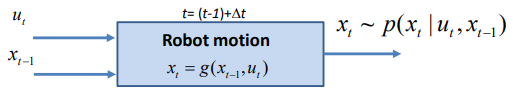
\includegraphics{images/fig3-2-probatilistic_robot_motion.PNG}
\end{figure}
Fig. 1: Inputs and outputs of a probabilistic motion model.

Different definitions for the \(g(\cdot)\) function lead to different
probabilistic motion models, like the velocity motion model explored
here.

    \hypertarget{the-model}{%
\subsection{3.2.1 The model}\label{the-model}}

The \emph{velocity motion model} is mainly used for motion planning,
where the details of the robot's movement are of importance and odometry
information is not available (\emph{e.g.} no wheel encoders are
available).

This motion model is characterized by the use of two velocities to
control the robot's movement: \textbf{linear velocity} \(v\) and
\textbf{angular velocity} \(w\). Therefore, during the following
sections, the movement commands will be of the form:

\[u_t = \begin{bmatrix} v_t \\ w_t \end{bmatrix}, \, \, \, u_t \sim N(\overline{u},\Sigma_{u_t})\]

The velocity motion model defines the function \(g(\cdot)\) as:

\[g(x_{t-1},u_t)=x_{t-1} \oplus \Delta x_t, \, \, \,
x_{t-1}\sim N (\overline{x}_{t-1},\Sigma_{x_{t-1}})\]

being \(\Delta_{x_t}=[\Delta_{x_t}, \Delta_{y_t}, \Delta_{\theta_t}]\)
(assuming w and v constant): -
\(\Delta x_t = \frac{v}{w} \sin(w\Delta t)\) -
\(\Delta y_t = \frac{v}{w} [1-\cos(w\Delta t)]\) -
\(\Delta \theta_t = w\Delta t\)

Note that \(g(x_{t-1},u_t)=x_{t-1} \oplus \Delta x_t\) \textbf{is not a
linear operation!}

In this way, this motion model is characterized by the following
equations, depending on the value of the angular velocity \(w\) (note
that a division by zero would appear in the first case with \(w=0\)):

\begin{itemize}
\item
  If \(w \neq 0\):

  \[
        \begin{bmatrix}
        x_t \\
        y_t \\
        \theta_t \\ 
        \end{bmatrix} 
        = 
        \begin{bmatrix}
        x_{t-1} \\
        y_{t-1} \\
        \theta_{t-1} \\ 
        \end{bmatrix} 
        +
        \begin{bmatrix}
            -R \sin \theta_{t-1} + R \sin(\theta_{t-1} + \Delta \theta) \\ 
            R \cos \theta_{t-1} - R \cos(\theta_{t-1} + \Delta \theta)\\
            \Delta \theta
        \end{bmatrix}
    \]
\item
  If \(w = 0\):

  \[
       \begin{bmatrix}
        x_t \\
        y_t \\
        \theta_t \\ 
        \end{bmatrix} 
        = 
        \begin{bmatrix}
        x_{t-1} \\
        y_{t-1} \\
        \theta_{t-1} \\ 
        \end{bmatrix} 
        + v \cdot \Delta t
        \begin{bmatrix}
            \cos \theta_{t-1} \\ \sin \theta_{t-1} \\ 0
        \end{bmatrix}
    \]
\end{itemize}

with:

\begin{itemize}
\tightlist
\item
  \(v = w \cdot R\) \emph{R is also called the curvature radius}
\item
  \(\Delta \theta = w \cdot \Delta t\)
\end{itemize}

    \begin{tcolorbox}[breakable, size=fbox, boxrule=1pt, pad at break*=1mm,colback=cellbackground, colframe=cellborder]
\prompt{In}{incolor}{2}{\boxspacing}
\begin{Verbatim}[commandchars=\\\{\}]
\PY{o}{\PYZpc{}}\PY{k}{matplotlib} notebook

\PY{c+c1}{\PYZsh{} IMPORTS}
\PY{k+kn}{import} \PY{n+nn}{numpy} \PY{k}{as} \PY{n+nn}{np}
\PY{k+kn}{from} \PY{n+nn}{numpy} \PY{k+kn}{import} \PY{n}{random}
\PY{k+kn}{import} \PY{n+nn}{matplotlib}\PY{n+nn}{.}\PY{n+nn}{pyplot} \PY{k}{as} \PY{n+nn}{plt}

\PY{k+kn}{import} \PY{n+nn}{sys}
\PY{n}{sys}\PY{o}{.}\PY{n}{path}\PY{o}{.}\PY{n}{append}\PY{p}{(}\PY{l+s+s2}{\PYZdq{}}\PY{l+s+s2}{..}\PY{l+s+s2}{\PYZdq{}}\PY{p}{)}
\PY{k+kn}{from} \PY{n+nn}{utils}\PY{n+nn}{.}\PY{n+nn}{DrawRobot} \PY{k+kn}{import} \PY{n}{DrawRobot}
\PY{k+kn}{from} \PY{n+nn}{utils}\PY{n+nn}{.}\PY{n+nn}{PlotEllipse} \PY{k+kn}{import} \PY{n}{PlotEllipse}
\end{Verbatim}
\end{tcolorbox}

    \hypertarget{assignment-1-the-model-in-action}{%
\subsubsection{\texorpdfstring{\textbf{{ASSIGNMENT 1: The model in
action}}}{ASSIGNMENT 1: The model in action}}\label{assignment-1-the-model-in-action}}

Modify the following \texttt{next\_pose()} function, used in the
\texttt{VelocityRobot} class below, which computes the next pose \(x_t\)
of a robot given: - its previous pose \(x_{t-1}\), - the velocity
movement command \(u=[v,w]^T\), and - a lapse of time \(\Delta t\).

Concretly you have to complete the if-else statement that takes into
account when the robot moves in an straight line so \(w = 0\).
\emph{Note: you don't have to modify the \texttt{None} in the function
header nor in the \texttt{if\ cov\ is\ not\ None:} condition.}

Remark that at this point \textbf{we are not taking into account
uncertainty in the system}: neither from the initial pose
(\(\Sigma_{x_{t-1}}\)) nor the movement \((v, w)\) (\(\Sigma_{u_{t}}\)).

\textbf{Example}

\begin{figure}
\centering
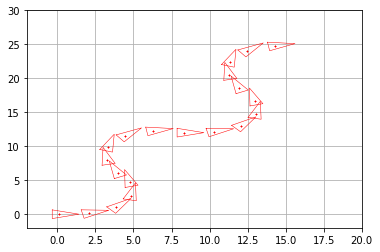
\includegraphics{images/fig3-2-1.png}
\end{figure}
Fig. 2: Route of our robot.

    \begin{tcolorbox}[breakable, size=fbox, boxrule=1pt, pad at break*=1mm,colback=cellbackground, colframe=cellborder]
\prompt{In}{incolor}{3}{\boxspacing}
\begin{Verbatim}[commandchars=\\\{\}]
\PY{k}{def} \PY{n+nf}{next\PYZus{}pose}\PY{p}{(}\PY{n}{x}\PY{p}{,} \PY{n}{u}\PY{p}{,} \PY{n}{dt}\PY{p}{,} \PY{n}{cov}\PY{o}{=}\PY{k+kc}{None}\PY{p}{)}\PY{p}{:}
    \PY{l+s+sd}{\PYZsq{}\PYZsq{}\PYZsq{} This function takes pose x and transform it according to the motion u=[v,w]\PYZsq{}}
\PY{l+s+sd}{        applying the differential drive model.}

\PY{l+s+sd}{        Args:}
\PY{l+s+sd}{            x: current pose}
\PY{l+s+sd}{            u: differential command as a vector [v, w]\PYZsq{}}
\PY{l+s+sd}{            dt: Time interval in which the movement occurs}
\PY{l+s+sd}{            cov: covariance of our movement. If not None, then add gaussian noise}
\PY{l+s+sd}{    \PYZsq{}\PYZsq{}\PYZsq{}}
    \PY{k}{if} \PY{n}{cov} \PY{o+ow}{is} \PY{o+ow}{not} \PY{k+kc}{None}\PY{p}{:}        
        \PY{n}{u} \PY{o}{+}\PY{o}{=} \PY{n}{np}\PY{o}{.}\PY{n}{sqrt}\PY{p}{(}\PY{n}{cov}\PY{p}{)} \PY{o}{@} \PY{n}{random}\PY{o}{.}\PY{n}{randn}\PY{p}{(}\PY{l+m+mi}{2}\PY{p}{,} \PY{l+m+mi}{1}\PY{p}{)}
        \PY{c+c1}{\PYZsh{}u = np.random.multivariate\PYZus{}normal(u.flatten(),cov)}

    \PY{k}{if} \PY{n}{u}\PY{p}{[}\PY{l+m+mi}{1}\PY{p}{]} \PY{o}{==} \PY{l+m+mi}{0}\PY{p}{:} \PY{c+c1}{\PYZsh{}linear motion w=0}
        
        
        \PY{n}{next\PYZus{}x} \PY{o}{=} \PY{n}{np}\PY{o}{.}\PY{n}{vstack}\PY{p}{(}\PY{p}{[}\PY{n}{x}\PY{p}{[}\PY{l+m+mi}{0}\PY{p}{]} \PY{o}{+} \PY{n}{u}\PY{p}{[}\PY{l+m+mi}{0}\PY{p}{]}\PY{o}{*}\PY{n}{dt}\PY{o}{*}\PY{n}{np}\PY{o}{.}\PY{n}{cos}\PY{p}{(}\PY{n}{x}\PY{p}{[}\PY{l+m+mi}{2}\PY{p}{]}\PY{p}{)}\PY{p}{,}
                            \PY{n}{x}\PY{p}{[}\PY{l+m+mi}{1}\PY{p}{]} \PY{o}{+} \PY{n}{u}\PY{p}{[}\PY{l+m+mi}{0}\PY{p}{]}\PY{o}{*}\PY{n}{dt}\PY{o}{*}\PY{n}{np}\PY{o}{.}\PY{n}{sin}\PY{p}{(}\PY{n}{x}\PY{p}{[}\PY{l+m+mi}{2}\PY{p}{]}\PY{p}{)}\PY{p}{,}
                            \PY{n}{X}\PY{p}{[}\PY{l+m+mi}{2}\PY{p}{]}\PY{p}{]}\PY{p}{)}
    \PY{k}{else}\PY{p}{:} \PY{c+c1}{\PYZsh{}Non\PYZhy{}linear motion w=!0}
        \PY{n}{R} \PY{o}{=} \PY{n}{u}\PY{p}{[}\PY{l+m+mi}{0}\PY{p}{]}\PY{o}{/}\PY{n}{u}\PY{p}{[}\PY{l+m+mi}{1}\PY{p}{]} \PY{c+c1}{\PYZsh{}v/w=r is the curvature radius}
        
        \PY{n}{dTheta} \PY{o}{=} \PY{n}{u}\PY{p}{[}\PY{l+m+mi}{1}\PY{p}{]} \PY{o}{*} \PY{n}{dt}
        \PY{n}{next\PYZus{}x} \PY{o}{=} \PY{n}{np}\PY{o}{.}\PY{n}{vstack}\PY{p}{(}\PY{p}{[}\PY{n}{x}\PY{p}{[}\PY{l+m+mi}{0}\PY{p}{]} \PY{o}{+} \PY{p}{(}\PY{o}{\PYZhy{}}\PY{n}{R}\PY{o}{*}\PY{n}{np}\PY{o}{.}\PY{n}{sin}\PY{p}{(}\PY{n}{x}\PY{p}{[}\PY{l+m+mi}{2}\PY{p}{]}\PY{p}{)} \PY{o}{+} \PY{n}{R}\PY{o}{*}\PY{n}{np}\PY{o}{.}\PY{n}{sin}\PY{p}{(}\PY{n}{x}\PY{p}{[}\PY{l+m+mi}{2}\PY{p}{]} \PY{o}{+} \PY{n}{dTheta}\PY{p}{)}\PY{p}{)}\PY{p}{,}
                            \PY{n}{x}\PY{p}{[}\PY{l+m+mi}{1}\PY{p}{]} \PY{o}{+} \PY{p}{(}\PY{n}{R}\PY{o}{*}\PY{n}{np}\PY{o}{.}\PY{n}{cos}\PY{p}{(}\PY{n}{x}\PY{p}{[}\PY{l+m+mi}{2}\PY{p}{]}\PY{p}{)} \PY{o}{\PYZhy{}} \PY{n}{R}\PY{o}{*}\PY{n}{np}\PY{o}{.}\PY{n}{cos}\PY{p}{(}\PY{n}{x}\PY{p}{[}\PY{l+m+mi}{2}\PY{p}{]} \PY{o}{+} \PY{n}{dTheta}\PY{p}{)}\PY{p}{)}\PY{p}{,}
                            \PY{n}{x}\PY{p}{[}\PY{l+m+mi}{2}\PY{p}{]} \PY{o}{+} \PY{n}{dTheta}\PY{p}{]}\PY{p}{)}

    \PY{k}{return} \PY{n}{next\PYZus{}x}
\end{Verbatim}
\end{tcolorbox}

    \begin{tcolorbox}[breakable, size=fbox, boxrule=1pt, pad at break*=1mm,colback=cellbackground, colframe=cellborder]
\prompt{In}{incolor}{4}{\boxspacing}
\begin{Verbatim}[commandchars=\\\{\}]
\PY{k}{class} \PY{n+nc}{VelocityRobot}\PY{p}{(}\PY{n+nb}{object}\PY{p}{)}\PY{p}{:}
    \PY{l+s+sd}{\PYZdq{}\PYZdq{}\PYZdq{} Mobile robot implementation that uses velocity commands.}
\PY{l+s+sd}{    }
\PY{l+s+sd}{        Attr:}
\PY{l+s+sd}{            pose: expected pose of the robot in the real world (without taking account noise)}
\PY{l+s+sd}{            dt: Duration of each step in seconds}
\PY{l+s+sd}{    \PYZdq{}\PYZdq{}\PYZdq{}}    
    \PY{k}{def} \PY{n+nf+fm}{\PYZus{}\PYZus{}init\PYZus{}\PYZus{}}\PY{p}{(}\PY{n+nb+bp}{self}\PY{p}{,} \PY{n}{mean}\PY{p}{,} \PY{n}{dt}\PY{p}{)}\PY{p}{:}
        \PY{n+nb+bp}{self}\PY{o}{.}\PY{n}{pose} \PY{o}{=} \PY{n}{mean}
        \PY{n+nb+bp}{self}\PY{o}{.}\PY{n}{dt} \PY{o}{=} \PY{n}{dt}
        
    \PY{k}{def} \PY{n+nf}{step}\PY{p}{(}\PY{n+nb+bp}{self}\PY{p}{,} \PY{n}{u}\PY{p}{)}\PY{p}{:}
        \PY{n+nb+bp}{self}\PY{o}{.}\PY{n}{pose} \PY{o}{=} \PY{n}{next\PYZus{}pose}\PY{p}{(}\PY{n+nb+bp}{self}\PY{o}{.}\PY{n}{pose}\PY{p}{,} \PY{n}{u}\PY{p}{,} \PY{n+nb+bp}{self}\PY{o}{.}\PY{n}{dt}\PY{p}{)}
        
    \PY{k}{def} \PY{n+nf}{draw}\PY{p}{(}\PY{n+nb+bp}{self}\PY{p}{,} \PY{n}{fig}\PY{p}{,} \PY{n}{ax}\PY{p}{)}\PY{p}{:}
        \PY{n}{DrawRobot}\PY{p}{(}\PY{n}{fig}\PY{p}{,} \PY{n}{ax}\PY{p}{,} \PY{n+nb+bp}{self}\PY{o}{.}\PY{n}{pose}\PY{p}{)}
\end{Verbatim}
\end{tcolorbox}

    \textbf{Test the movement of your robot} using the demo below.

    \begin{tcolorbox}[breakable, size=fbox, boxrule=1pt, pad at break*=1mm,colback=cellbackground, colframe=cellborder]
\prompt{In}{incolor}{5}{\boxspacing}
\begin{Verbatim}[commandchars=\\\{\}]
\PY{k}{def} \PY{n+nf}{main}\PY{p}{(}\PY{n}{robot}\PY{p}{,} \PY{n}{nSteps}\PY{p}{)}\PY{p}{:}
          
    \PY{n}{v} \PY{o}{=} \PY{l+m+mi}{1} \PY{c+c1}{\PYZsh{} Linear Velocity }
    \PY{n}{l} \PY{o}{=} \PY{l+m+mf}{0.5} \PY{c+c1}{\PYZsh{}Half the width of the robot}
        
    \PY{c+c1}{\PYZsh{} MATPLOTLIB}
    \PY{n}{fig}\PY{p}{,} \PY{n}{ax} \PY{o}{=} \PY{n}{plt}\PY{o}{.}\PY{n}{subplots}\PY{p}{(}\PY{p}{)}
    \PY{n}{plt}\PY{o}{.}\PY{n}{ion}\PY{p}{(}\PY{p}{)}
    \PY{n}{fig}\PY{o}{.}\PY{n}{canvas}\PY{o}{.}\PY{n}{draw}\PY{p}{(}\PY{p}{)}
    \PY{n}{plt}\PY{o}{.}\PY{n}{xlim}\PY{p}{(}\PY{p}{(}\PY{o}{\PYZhy{}}\PY{l+m+mi}{2}\PY{p}{,} \PY{l+m+mi}{20}\PY{p}{)}\PY{p}{)}
    \PY{n}{plt}\PY{o}{.}\PY{n}{ylim}\PY{p}{(}\PY{p}{(}\PY{o}{\PYZhy{}}\PY{l+m+mi}{2}\PY{p}{,} \PY{l+m+mi}{30}\PY{p}{)}\PY{p}{)}
    
    \PY{n}{plt}\PY{o}{.}\PY{n}{grid}\PY{p}{(}\PY{p}{)}
        
    \PY{c+c1}{\PYZsh{} MAIN LOOP}
    \PY{k}{for} \PY{n}{k} \PY{o+ow}{in} \PY{n+nb}{range}\PY{p}{(}\PY{l+m+mi}{1}\PY{p}{,} \PY{n}{nSteps} \PY{o}{+} \PY{l+m+mi}{1}\PY{p}{)}\PY{p}{:}
        \PY{c+c1}{\PYZsh{}control is a wiggle with constant linear velocity}
        \PY{n}{u} \PY{o}{=} \PY{n}{np}\PY{o}{.}\PY{n}{vstack}\PY{p}{(}\PY{p}{(}\PY{n}{v}\PY{p}{,} \PY{n}{np}\PY{o}{.}\PY{n}{pi} \PY{o}{/} \PY{l+m+mi}{10} \PY{o}{*} \PY{n}{np}\PY{o}{.}\PY{n}{sin}\PY{p}{(}\PY{l+m+mi}{4} \PY{o}{*} \PY{n}{np}\PY{o}{.}\PY{n}{pi} \PY{o}{*} \PY{n}{k}\PY{o}{/}\PY{n}{nSteps}\PY{p}{)}\PY{p}{)}\PY{p}{)}
        
        \PY{n}{robot}\PY{o}{.}\PY{n}{step}\PY{p}{(}\PY{n}{u}\PY{p}{)}   
        
        \PY{c+c1}{\PYZsh{}draw occasionally}
        \PY{k}{if} \PY{p}{(}\PY{n}{k}\PY{o}{\PYZhy{}}\PY{l+m+mi}{1}\PY{p}{)}\PY{o}{\PYZpc{}}\PY{k}{20} == 0:
            \PY{n}{robot}\PY{o}{.}\PY{n}{draw}\PY{p}{(}\PY{n}{fig}\PY{p}{,} \PY{n}{ax}\PY{p}{)}
            \PY{n}{fig}\PY{o}{.}\PY{n}{canvas}\PY{o}{.}\PY{n}{draw}\PY{p}{(}\PY{p}{)}
            \PY{n}{plt}\PY{o}{.}\PY{n}{pause}\PY{p}{(}\PY{l+m+mf}{0.1}\PY{p}{)}
\end{Verbatim}
\end{tcolorbox}

    \begin{tcolorbox}[breakable, size=fbox, boxrule=1pt, pad at break*=1mm,colback=cellbackground, colframe=cellborder]
\prompt{In}{incolor}{6}{\boxspacing}
\begin{Verbatim}[commandchars=\\\{\}]
\PY{c+c1}{\PYZsh{} RUN }
\PY{n}{dT} \PY{o}{=} \PY{l+m+mf}{0.1} \PY{c+c1}{\PYZsh{} time steps size}
\PY{n}{pose} \PY{o}{=} \PY{n}{np}\PY{o}{.}\PY{n}{vstack}\PY{p}{(}\PY{p}{[}\PY{l+m+mf}{0.}\PY{p}{,} \PY{l+m+mf}{0.}\PY{p}{,} \PY{l+m+mf}{0.}\PY{p}{]}\PY{p}{)}

\PY{n}{robot} \PY{o}{=} \PY{n}{VelocityRobot}\PY{p}{(}\PY{n}{pose}\PY{p}{,} \PY{n}{dT}\PY{p}{)}
\PY{n}{main}\PY{p}{(}\PY{n}{robot}\PY{p}{,} \PY{n}{nSteps}\PY{o}{=}\PY{l+m+mi}{400}\PY{p}{)}
\end{Verbatim}
\end{tcolorbox}

\begin{figure}
\centering
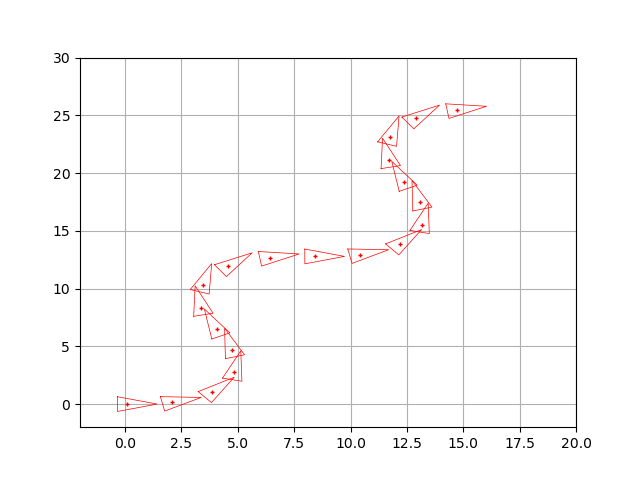
\includegraphics{returns/321.png}
\end{figure}

    
    \hypertarget{propagating-uncertainty}{%
\subsection{3.2.2 Propagating
uncertainty}\label{propagating-uncertainty}}

In the previous section we introduced how to compute the robot pose
\(x\) at time instant \(t\) by applying a control action \(u_t\).
However, as we know, this process has different sources of uncertainty
that need to be modeled someway.

To deal with this we will consider two Gaussian distributions: - the
\textbf{robot pose} modeled as
\(x_t \sim(\overline{x}_t, \Sigma_{x_t})\) at time \(t\). Similarly, for
the \textbf{previous pose} at \(t-1\) we have
\(x_{t-1} \sim(\overline{x}_{t-1}, \Sigma_{x_{t-1}})\), - and the
\textbf{movement command} as \(u_t\sim(\overline{u}_t, \Sigma_{u_t})\),
being applied during an interval of time \(\Delta t\).

In this way, after a motion command we can retrieve the probability
distribution \(x_t\) modeling the new robot pose as:

\begin{itemize}
\item
  \textbf{Mean:}
  \[\overline{x}_t = \overline{x}_{t-1} \oplus \overline{u}_t = g(\overline{x}_{t-1}, \overline{u}_t)\]
\item
  \textbf{Covariance:}
  \[\Sigma_{x_t} =  \frac{\partial g}{\partial x_{t-1}} \cdot \Sigma_{x_{t-1}} \cdot {\frac{\partial g}{\partial x_{t-1}}}^T + \frac{\partial g}{\partial u_{t}} \cdot \Sigma_{u_t} \cdot {\frac{\partial g}{\partial u_{t}}}^T \\[10pt]\]
  where \(\partial g / \partial x_{t-1}\) and
  \(\partial g / \partial u_{t}\) are the jacobians of our motion model
  evaluated at the previous pose \(x_{t-1}\) and the current command
  \(u_t\), and the covariance matrix of this movement (\(\Sigma_{u_t}\))
  is defined as seen below. Typically, it is constant during robot
  motion:\(\\[10pt]\) \[ 
    \Sigma_{u_t} = \begin{bmatrix}
            \sigma_v^2 & 0 \\
            0 &  \sigma_w^2
        \end{bmatrix}
  \]
\end{itemize}

    \hypertarget{optional}{%
\subsection{\texorpdfstring{{OPTIONAL}}{OPTIONAL}}\label{optional}}

{Write a Markdown cell containing the Jacobians ecuations
aforementioned.}

    {\textbf{\emph{END OF OPTIONAL PART}}}

    \hypertarget{assignment-2-adding-uncertainty}{%
\subsubsection{\texorpdfstring{\textbf{{ASSIGNMENT 2: Adding
uncertainty}}}{ASSIGNMENT 2: Adding uncertainty}}\label{assignment-2-adding-uncertainty}}

Now we will include uncertainty to the previous assignment, changing the
behavior of the robot class \texttt{VelocityRobot()} you have
implemented.

In contrast to the noisy robot \texttt{NoisyRobot()} in notebook 3.1, we
will use the equations of the velocity motion model and their respective
Jacobians to keep track of how confident we are of the robot's pose
(i.e.~the robot's pose \(x_t\) now is also a gaussian distribution).

Consider the following: - the expected robot pose \(\overline{x}_t\) is
stored in \texttt{self.pose}. - the covariance matrix of the robot pose
\(\Sigma_{x_t}\) is named \texttt{P\_t} in the code, - the covariance
matrix of the robot motion \(\Sigma_{u_t}\) is \texttt{Q}, and - the
jacobians of our motion model \(\partial g / \partial x_{t-1}\) and
\(\partial g / \partial u_{t}\) are \texttt{JacF\_x} and
\texttt{JacF\_u}.

    \textbf{First} Complete the following code calculating the covariance
matrix \(\Sigma_{x_t}\) (\texttt{P\_t}). That is, you have to: -
Implement the jacobians \texttt{JacF\_x} and \texttt{JacF\_u}, which
depend on the angular velocity \(w\), and - Compute the covariance
matrix \texttt{P\_t}using such jacobians, the current covariance of the
pose \texttt{P}, and the covariance of the motion \texttt{Q}.

    \begin{tcolorbox}[breakable, size=fbox, boxrule=1pt, pad at break*=1mm,colback=cellbackground, colframe=cellborder]
\prompt{In}{incolor}{7}{\boxspacing}
\begin{Verbatim}[commandchars=\\\{\}]
\PY{k}{def} \PY{n+nf}{next\PYZus{}covariance}\PY{p}{(}\PY{n}{x}\PY{p}{,} \PY{n}{P}\PY{p}{,} \PY{n}{Q}\PY{p}{,} \PY{n}{u}\PY{p}{,} \PY{n}{dt}\PY{p}{)}\PY{p}{:}
    \PY{l+s+sd}{\PYZsq{}\PYZsq{}\PYZsq{} Compute the covariance of a robot following the velocity motion model}

\PY{l+s+sd}{        Args:}
\PY{l+s+sd}{            x: current pose (before movement)}
\PY{l+s+sd}{            u: differential command as a vector [v, w]\PYZsq{}\PYZsq{}}
\PY{l+s+sd}{            dt: Time interval in which the movement occurs}
\PY{l+s+sd}{            P: current covariance of the pose}
\PY{l+s+sd}{            Q: covariance of our movement.}
\PY{l+s+sd}{    \PYZsq{}\PYZsq{}\PYZsq{}}    
    \PY{c+c1}{\PYZsh{} Aliases}
    \PY{n}{v} \PY{o}{=} \PY{n}{u}\PY{p}{[}\PY{l+m+mi}{0}\PY{p}{,} \PY{l+m+mi}{0}\PY{p}{]}
    \PY{n}{w} \PY{o}{=} \PY{n}{u}\PY{p}{[}\PY{l+m+mi}{1}\PY{p}{,} \PY{l+m+mi}{0}\PY{p}{]}

    \PY{n}{sx}\PY{p}{,} \PY{n}{cx} \PY{o}{=} \PY{n}{np}\PY{o}{.}\PY{n}{sin}\PY{p}{(}\PY{n}{x}\PY{p}{[}\PY{l+m+mi}{2}\PY{p}{,} \PY{l+m+mi}{0}\PY{p}{]}\PY{p}{)}\PY{p}{,} \PY{n}{np}\PY{o}{.}\PY{n}{cos}\PY{p}{(}\PY{n}{x}\PY{p}{[}\PY{l+m+mi}{2}\PY{p}{,} \PY{l+m+mi}{0}\PY{p}{]}\PY{p}{)} \PY{c+c1}{\PYZsh{}sin and cos for the previous robot heading}
    \PY{n}{si}\PY{p}{,} \PY{n}{ci} \PY{o}{=} \PY{n}{np}\PY{o}{.}\PY{n}{sin}\PY{p}{(}\PY{n}{u}\PY{p}{[}\PY{l+m+mi}{1}\PY{p}{,} \PY{l+m+mi}{0}\PY{p}{]}\PY{o}{*}\PY{n}{dt}\PY{p}{)}\PY{p}{,} \PY{n}{np}\PY{o}{.}\PY{n}{cos}\PY{p}{(}\PY{n}{u}\PY{p}{[}\PY{l+m+mi}{1}\PY{p}{,} \PY{l+m+mi}{0}\PY{p}{]}\PY{o}{*}\PY{n}{dt}\PY{p}{)} \PY{c+c1}{\PYZsh{}sin and cos for the heading increment}
    \PY{n}{R} \PY{o}{=} \PY{n}{u}\PY{p}{[}\PY{l+m+mi}{0}\PY{p}{,} \PY{l+m+mi}{0}\PY{p}{]}\PY{o}{/}\PY{n}{u}\PY{p}{[}\PY{l+m+mi}{1}\PY{p}{,} \PY{l+m+mi}{0}\PY{p}{]} \PY{c+c1}{\PYZsh{}v/w Curvature radius}

    \PY{k}{if} \PY{n}{u}\PY{p}{[}\PY{l+m+mi}{1}\PY{p}{,} \PY{l+m+mi}{0}\PY{p}{]} \PY{o}{==} \PY{l+m+mi}{0}\PY{p}{:}  \PY{c+c1}{\PYZsh{}linear motion w=0 \PYZhy{}\PYZhy{}\PYZgt{} R = infinite}
        \PY{c+c1}{\PYZsh{}TODO JACOBIAN HERE}
        \PY{n}{JacF\PYZus{}x} \PY{o}{=} \PY{n}{np}\PY{o}{.}\PY{n}{array}\PY{p}{(}\PY{p}{[}
            \PY{p}{[}\PY{l+m+mi}{1}\PY{p}{,}\PY{l+m+mi}{0}\PY{p}{,} \PY{o}{\PYZhy{}}\PY{n}{v}\PY{o}{*}\PY{n}{dt}\PY{o}{*}\PY{n}{sx}\PY{p}{]}\PY{p}{,}
            \PY{p}{[}\PY{l+m+mi}{0}\PY{p}{,}\PY{l+m+mi}{1}\PY{p}{,} \PY{n}{v}\PY{o}{*}\PY{n}{dt}\PY{o}{*}\PY{n}{cx}\PY{p}{]}\PY{p}{,}
            \PY{p}{[}\PY{l+m+mi}{0}\PY{p}{,}\PY{l+m+mi}{0}\PY{p}{,}\PY{l+m+mi}{1}\PY{p}{]}
        \PY{p}{]}\PY{p}{)}
        \PY{n}{JacF\PYZus{}u} \PY{o}{=} \PY{n}{np}\PY{o}{.}\PY{n}{array}\PY{p}{(}\PY{p}{[}
            \PY{p}{[}\PY{n}{dt}\PY{o}{*}\PY{n}{cx}\PY{p}{,} \PY{n}{dt}\PY{o}{*}\PY{n}{sx}\PY{p}{,} \PY{l+m+mi}{0}\PY{p}{]}\PY{p}{,}
            \PY{p}{[}\PY{l+m+mi}{0}\PY{p}{,}\PY{l+m+mi}{0}\PY{p}{,}\PY{l+m+mi}{0}\PY{p}{]}
        \PY{p}{]}\PY{p}{)}
    \PY{k}{else}\PY{p}{:} \PY{c+c1}{\PYZsh{}Non\PYZhy{}linear motion w=!0}
        \PY{c+c1}{\PYZsh{} TODO JACOBIAN HERE}
        \PY{n}{JacF\PYZus{}x} \PY{o}{=} \PY{n}{np}\PY{o}{.}\PY{n}{array}\PY{p}{(}\PY{p}{[}
            \PY{p}{[}\PY{l+m+mi}{1}\PY{p}{,}\PY{l+m+mi}{0}\PY{p}{,} \PY{n}{R}\PY{o}{*}\PY{p}{(}\PY{o}{\PYZhy{}}\PY{n}{sx}\PY{o}{*}\PY{n}{si} \PY{o}{\PYZhy{}}\PY{n}{cx}\PY{o}{*}\PY{p}{(}\PY{l+m+mi}{1}\PY{o}{\PYZhy{}}\PY{n}{ci}\PY{p}{)}\PY{p}{)} \PY{p}{]}\PY{p}{,}
            \PY{p}{[}\PY{l+m+mi}{0}\PY{p}{,}\PY{l+m+mi}{1}\PY{p}{,} \PY{n}{R}\PY{o}{*}\PY{p}{(}\PY{n}{cx}\PY{o}{*}\PY{n}{si} \PY{o}{\PYZhy{}}\PY{n}{sx}\PY{o}{*}\PY{p}{(}\PY{l+m+mi}{1}\PY{o}{\PYZhy{}}\PY{n}{ci}\PY{p}{)}\PY{p}{)}\PY{p}{]}\PY{p}{,}
            \PY{p}{[}\PY{l+m+mi}{0}\PY{p}{,}\PY{l+m+mi}{0}\PY{p}{,}\PY{l+m+mi}{1}\PY{p}{]}
        \PY{p}{]}\PY{p}{)}

        \PY{n}{JacF\PYZus{}u} \PY{o}{=} \PY{p}{(}
            \PY{n}{np}\PY{o}{.}\PY{n}{array}\PY{p}{(}\PY{p}{[}
                \PY{p}{[}\PY{n}{cx}\PY{o}{*}\PY{n}{si} \PY{o}{\PYZhy{}} \PY{n}{sx}\PY{o}{*}\PY{p}{(}\PY{l+m+mi}{1}\PY{o}{\PYZhy{}}\PY{n}{ci}\PY{p}{)}\PY{p}{,} \PY{n}{R}\PY{o}{*}\PY{p}{(}\PY{n}{cx}\PY{o}{*}\PY{n}{ci} \PY{o}{\PYZhy{}} \PY{n}{sx}\PY{o}{*}\PY{n}{si}\PY{p}{)}\PY{p}{]}\PY{p}{,}
                \PY{p}{[}\PY{n}{sx}\PY{o}{*}\PY{n}{si} \PY{o}{+} \PY{n}{cx}\PY{o}{*}\PY{p}{(}\PY{l+m+mi}{1}\PY{o}{\PYZhy{}}\PY{n}{ci}\PY{p}{)}\PY{p}{,} \PY{n}{R}\PY{o}{*}\PY{p}{(}\PY{n}{sx}\PY{o}{*}\PY{n}{ci} \PY{o}{\PYZhy{}} \PY{n}{cx}\PY{o}{*}\PY{n}{si}\PY{p}{)}\PY{p}{]}\PY{p}{,}
                \PY{p}{[}\PY{l+m+mi}{0}\PY{p}{,} \PY{l+m+mi}{1}\PY{p}{]}
            \PY{p}{]}\PY{p}{)}\PY{o}{@}
            \PY{n}{np}\PY{o}{.}\PY{n}{array}\PY{p}{(}\PY{p}{[}
                \PY{p}{[}\PY{l+m+mi}{1}\PY{o}{/}\PY{n}{w}\PY{p}{,} \PY{o}{\PYZhy{}}\PY{n}{v}\PY{o}{/}\PY{n}{w}\PY{o}{*}\PY{o}{*}\PY{l+m+mi}{2}\PY{p}{]}\PY{p}{,}
                \PY{p}{[}\PY{l+m+mi}{0}\PY{p}{,} \PY{n}{dt}\PY{p}{]}
            \PY{p}{]}\PY{p}{)}
        \PY{p}{)}
    \PY{c+c1}{\PYZsh{}prediction steps        }
    
    \PY{n}{Pt\PYZus{}x} \PY{o}{=} \PY{p}{(} \PY{n}{JacF\PYZus{}x} \PY{o}{@} \PY{n}{P} \PY{o}{@} \PY{n}{JacF\PYZus{}x}\PY{o}{.}\PY{n}{T} \PY{p}{)}
    
    \PY{n}{Pt\PYZus{}u} \PY{o}{=} \PY{p}{(} \PY{n}{JacF\PYZus{}u} \PY{o}{@} \PY{n}{Q} \PY{o}{@} \PY{n}{JacF\PYZus{}u}\PY{o}{.}\PY{n}{T} \PY{p}{)}
    
    \PY{n}{Pt} \PY{o}{=}  \PY{n}{Pt\PYZus{}x} \PY{o}{+} \PY{n}{Pt\PYZus{}u}
    
    \PY{k}{return} \PY{n}{Pt}
\end{Verbatim}
\end{tcolorbox}

    \textbf{Then}, complete the methods:

\begin{itemize}
\tightlist
\item
  \texttt{step()} to get the true robot pose (ground-truth) using the
  \(Q\) matrix (recall the \texttt{next\_pose()} function you defined
  before and its fourth input argument),
\item
  and the \texttt{draw()} one to plot an ellipse representing the
  uncertainty about the robot pose centered at the expected robot pose
  (\texttt{self.pose}) as well as marks representing the ground truth
  poses.
\end{itemize}

\textbf{Example}

\begin{figure}
\centering
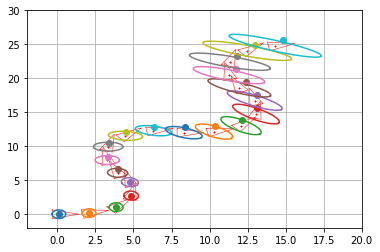
\includegraphics{images/fig3-2-2.png}
\end{figure}
Fig. 3: Movement of a robot using velocity commands. Representing the
expected pose (in red), the true pose (as dots) and the confidence
ellipse.

    \begin{tcolorbox}[breakable, size=fbox, boxrule=1pt, pad at break*=1mm,colback=cellbackground, colframe=cellborder]
\prompt{In}{incolor}{8}{\boxspacing}
\begin{Verbatim}[commandchars=\\\{\}]
\PY{k}{class} \PY{n+nc}{NoisyVelocityRobot}\PY{p}{(}\PY{n}{VelocityRobot}\PY{p}{)}\PY{p}{:}
    \PY{l+s+sd}{\PYZdq{}\PYZdq{}\PYZdq{} Mobile robot implementation that uses velocity commands.}
\PY{l+s+sd}{       }
\PY{l+s+sd}{        Attr:}
\PY{l+s+sd}{            [...]: Inherited from VelocityRobot}
\PY{l+s+sd}{            true\PYZus{}pose: expected pose of the robot in the real world (noisy)}
\PY{l+s+sd}{            cov\PYZus{}pose: Covariance of the pose at each step}
\PY{l+s+sd}{            cov\PYZus{}move: Covariance of each movement. It is a constant}

\PY{l+s+sd}{    \PYZdq{}\PYZdq{}\PYZdq{}}
    
    \PY{k}{def} \PY{n+nf+fm}{\PYZus{}\PYZus{}init\PYZus{}\PYZus{}}\PY{p}{(}\PY{n+nb+bp}{self}\PY{p}{,} \PY{n}{mean}\PY{p}{,} \PY{n}{cov\PYZus{}pose}\PY{p}{,} \PY{n}{cov\PYZus{}move}\PY{p}{,} \PY{n}{dt}\PY{p}{)}\PY{p}{:}
        \PY{n+nb}{super}\PY{p}{(}\PY{p}{)}\PY{o}{.}\PY{n+nf+fm}{\PYZus{}\PYZus{}init\PYZus{}\PYZus{}}\PY{p}{(}\PY{n}{mean}\PY{p}{,} \PY{n}{dt}\PY{p}{)}
        \PY{n+nb+bp}{self}\PY{o}{.}\PY{n}{true\PYZus{}pose} \PY{o}{=} \PY{n}{mean}
        \PY{n+nb+bp}{self}\PY{o}{.}\PY{n}{cov\PYZus{}pose} \PY{o}{=} \PY{n}{cov\PYZus{}pose}
        \PY{n+nb+bp}{self}\PY{o}{.}\PY{n}{cov\PYZus{}move} \PY{o}{=} \PY{n}{cov\PYZus{}move}
        
    \PY{k}{def} \PY{n+nf}{step}\PY{p}{(}\PY{n+nb+bp}{self}\PY{p}{,} \PY{n}{u}\PY{p}{)}\PY{p}{:}
        \PY{n+nb+bp}{self}\PY{o}{.}\PY{n}{cov\PYZus{}pose} \PY{o}{=} \PY{n}{next\PYZus{}covariance}\PY{p}{(}\PY{n+nb+bp}{self}\PY{o}{.}\PY{n}{pose}\PY{p}{,} \PY{n+nb+bp}{self}\PY{o}{.}\PY{n}{cov\PYZus{}pose}\PY{p}{,} \PY{n+nb+bp}{self}\PY{o}{.}\PY{n}{cov\PYZus{}move}\PY{p}{,} \PY{n}{u}\PY{p}{,} \PY{n+nb+bp}{self}\PY{o}{.}\PY{n}{dt}\PY{p}{)}
        
        \PY{n+nb}{super}\PY{p}{(}\PY{p}{)}\PY{o}{.}\PY{n}{step}\PY{p}{(}\PY{n}{u}\PY{p}{)}
        \PY{n+nb+bp}{self}\PY{o}{.}\PY{n}{true\PYZus{}pose} \PY{o}{=} \PY{n}{next\PYZus{}pose}\PY{p}{(}\PY{n+nb+bp}{self}\PY{o}{.}\PY{n}{true\PYZus{}pose}\PY{p}{,} \PY{n}{u}\PY{p}{,} \PY{n+nb+bp}{self}\PY{o}{.}\PY{n}{dt}\PY{p}{,} \PY{n}{cov}\PY{o}{=}\PY{n+nb+bp}{self}\PY{o}{.}\PY{n}{cov\PYZus{}move}\PY{p}{)}
        
    \PY{k}{def} \PY{n+nf}{draw}\PY{p}{(}\PY{n+nb+bp}{self}\PY{p}{,} \PY{n}{fig}\PY{p}{,} \PY{n}{ax}\PY{p}{)}\PY{p}{:}
        \PY{n+nb}{super}\PY{p}{(}\PY{p}{)}\PY{o}{.}\PY{n}{draw}\PY{p}{(}\PY{n}{fig}\PY{p}{,} \PY{n}{ax}\PY{p}{)}
        \PY{n}{el} \PY{o}{=} \PY{n}{PlotEllipse}\PY{p}{(}\PY{n}{fig}\PY{p}{,} \PY{n}{ax}\PY{p}{,} \PY{n+nb+bp}{self}\PY{o}{.}\PY{n}{pose}\PY{p}{,} \PY{n+nb+bp}{self}\PY{o}{.}\PY{n}{cov\PYZus{}pose}\PY{p}{)}
        \PY{n}{ax}\PY{o}{.}\PY{n}{plot}\PY{p}{(}\PY{n+nb+bp}{self}\PY{o}{.}\PY{n}{true\PYZus{}pose}\PY{p}{[}\PY{l+m+mi}{0}\PY{p}{,}\PY{l+m+mi}{0}\PY{p}{]}\PY{p}{,} \PY{n+nb+bp}{self}\PY{o}{.}\PY{n}{true\PYZus{}pose}\PY{p}{[}\PY{l+m+mi}{1}\PY{p}{,}\PY{l+m+mi}{0}\PY{p}{]}\PY{p}{,} \PY{l+s+s1}{\PYZsq{}}\PY{l+s+s1}{o}\PY{l+s+s1}{\PYZsq{}}\PY{p}{,} \PY{n}{color}\PY{o}{=}\PY{n}{el}\PY{p}{[}\PY{l+m+mi}{0}\PY{p}{]}\PY{o}{.}\PY{n}{get\PYZus{}color}\PY{p}{(}\PY{p}{)}\PY{p}{)}
\end{Verbatim}
\end{tcolorbox}

    Now, \textbf{try your implementation!}

    \begin{tcolorbox}[breakable, size=fbox, boxrule=1pt, pad at break*=1mm,colback=cellbackground, colframe=cellborder]
\prompt{In}{incolor}{27}{\boxspacing}
\begin{Verbatim}[commandchars=\\\{\}]
\PY{c+c1}{\PYZsh{} RUN}
\PY{n}{dT} \PY{o}{=} \PY{l+m+mf}{0.1} \PY{c+c1}{\PYZsh{} time steps size}

\PY{n}{SigmaV} \PY{o}{=} \PY{l+m+mf}{0.2} \PY{c+c1}{\PYZsh{}Standard deviation of the linear velocity. }
\PY{n}{SigmaW} \PY{o}{=} \PY{l+m+mf}{0.1} \PY{c+c1}{\PYZsh{}Standard deviation of the angular velocity}
\PY{n}{nSteps} \PY{o}{=} \PY{l+m+mi}{400} \PY{c+c1}{\PYZsh{}Number of motions}

\PY{n}{P} \PY{o}{=} \PY{n}{np}\PY{o}{.}\PY{n}{diag}\PY{p}{(}\PY{p}{[}\PY{l+m+mf}{0.2}\PY{p}{,} \PY{l+m+mf}{0.4}\PY{p}{,} \PY{l+m+mf}{0.}\PY{p}{]}\PY{p}{)} \PY{c+c1}{\PYZsh{}pose covariance matrix 3x3}
\PY{n}{Q} \PY{o}{=} \PY{n}{np}\PY{o}{.}\PY{n}{diag}\PY{p}{(}\PY{p}{[}\PY{n}{SigmaV}\PY{o}{*}\PY{o}{*}\PY{l+m+mi}{2}\PY{p}{,} \PY{n}{SigmaW}\PY{o}{*}\PY{o}{*}\PY{l+m+mi}{2}\PY{p}{]}\PY{p}{)} \PY{c+c1}{\PYZsh{}motion covariance matrix 2x2}

\PY{n}{robot} \PY{o}{=} \PY{n}{NoisyVelocityRobot}\PY{p}{(}\PY{n}{np}\PY{o}{.}\PY{n}{vstack}\PY{p}{(}\PY{p}{[}\PY{l+m+mf}{0.}\PY{p}{,} \PY{l+m+mf}{0.}\PY{p}{,} \PY{l+m+mf}{0.}\PY{p}{]}\PY{p}{)}\PY{p}{,} \PY{n}{P}\PY{p}{,} \PY{n}{Q}\PY{p}{,} \PY{n}{dT}\PY{p}{)}
\PY{n}{main}\PY{p}{(}\PY{n}{robot}\PY{p}{,} \PY{n}{nSteps}\PY{o}{=}\PY{n}{nSteps}\PY{p}{)}
\end{Verbatim}
\end{tcolorbox}

    
\begin{figure}
\centering
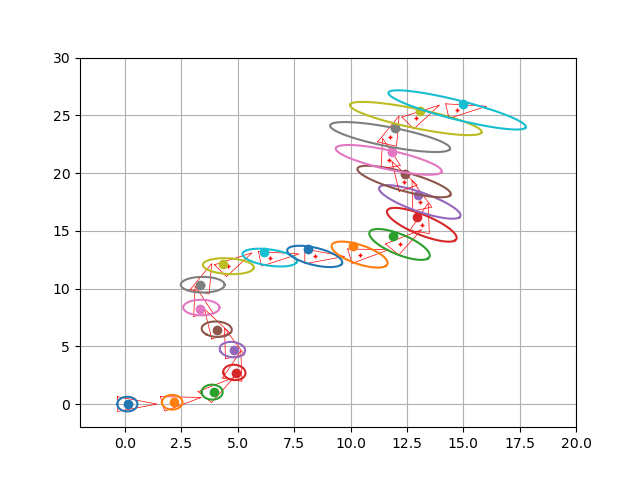
\includegraphics{returns/322.png}
\end{figure}
    
    \hypertarget{thinking-about-it-1}{%
\subsubsection{Thinking about it (1)}\label{thinking-about-it-1}}

Now that you have some experience with robot motion and the velocity
motion model, \textbf{answer the following questions}:

\begin{itemize}
\item
  Why do we need to consider two different cases when applying the
  \(g(\cdot)\) function, that is, calculating the new robot pose?

  Because we need to considerate the possibility that the robot is doing
  linear moves (w=0) or if it doesn't. For each case, the way to compute
  the next pose is different.
\item
  How many parameters compound the motion command \(u_t\) in this model?

  Two. Linear velocity (v) and angular velocity (w).
\item
  Why do we need to use Jacobians to propagate the uncertainty about the
  robot pose \(x_t\)?

  We use Jacobians to keep track of how confident we are of the robot's
  pose. (That is, robot's pose now follows a gaussian distribution).
\item
  What happens if you modify the covariance matrix \(\Sigma_{u_t}\)
  modeling the uncertainty in the motion command \(u_t\)? Try different
  values and discuss the results.

  When we increase SigmaV and/or SigmaW, the true pose of the robot is
  more distant from the perfect one. This distance increases as steps
  are taken. If we decrease those values, the true pose is near the
  perfect pose. If SigmaV and SigmaW are 0, both poses are equal in each
  step.
\end{itemize}


    % Add a bibliography block to the postdoc
    
    
    
\end{document}
